\documentclass[%
 aip,
 jcp,
%jmp,%
%bmf,%
 sd,%
%rsi,%
 amsmath,amssymb,
%preprint,%
%reprint,%
%author-year,%
%author-numerical,%
]{revtex4-1}
\maxdeadcycles=1000

\usepackage[colorlinks=true,allcolors=blue]{hyperref}
\usepackage{graphicx}
\usepackage{dcolumn}
\usepackage{bm}

\begin{document}


%\preprint{AIP/123-QED}

\title{Supporting Information: Coexistence Calculation Using the Isothermal-Isochoric Integration Method}

\author{S. Mostafa Razavi}
\email{sr87@uakron.edu}
\affiliation{Department of Chemical and Biomolecular Engineering, The University of Akron, Akron, Ohio 44325, USA}

\author{Richard A. Messerly}
\email{richard.messerly@nist.gov}
\affiliation{Thermodynamics Research Center, National Institute of Standards and Technology, Boulder, Colorado, 80305, USA}

\author{J. Richard Elliott}
\email{elliot1@uakron.edu}
\affiliation{Department of Chemical and Biomolecular Engineering, The University of Akron, Akron, Ohio 44325, USA}
\date{\today}

\maketitle


\section{Tables of Example Simulations Results}

\begin{table*}[!htbp]
\centering
\caption{Cassandra simulation results of TraPPE-UA ethane.}
\label{tab:NIST-VAL-C12-FTT}
\begin{ruledtabular}
\begin{tabular}{ccccccccccccccc}
[K] & [$\mathrm{g/cm^3}$] &  &  & \multicolumn{2}{c}{$[\frac{\mathrm{kcal}}{\mathrm{mol}}]$} & \multicolumn{2}{c}{$[\frac{\mathrm{kcal}}{\mathrm{mol}}]$} & \multicolumn{2}{c}{$[\frac{\mathrm{kcal}}{\mathrm{mol}}]$} &\multicolumn{2}{c}{$[\frac{\mathrm{kcal}}{\mathrm{mol}}]$} & \\
\hline
$T$ & $\rho$ & $Z$ & $\pm$ & $E^{\mathrm{tot}}$ & $\pm$ & $E^{\mathrm{bonded}}$ & $\pm$ & $E^{\mathrm{vdw}}$ & $\pm$ & $E^{\mathrm{intra}}$ & $\pm$ & N\\
\hline
260.24 & 0.4286 & 0.0793  & 0.017 & -1305.80 & 1.17 & 0.00 & 0.00 & -1271.80 & 1.17 & 0.00 & 0.00 & 600  \\
302.10 & 0.4286 & 0.6553  & 0.009 & -1275.90 & 0.32 & 0.00 & 0.00 & -1241.90 & 0.32 & 0.00 & 0.00 & 600  \\
236.27 & 0.4714 & 0.0533  & 0.038 & -1454.50 & 1.51 & 0.00 & 0.00 & -1417.10 & 1.51 & 0.00 & 0.00 & 600  \\
285.30 & 0.4714 & 0.9343  & 0.016 & -1415.70 & 0.56 & 0.00 & 0.00 & -1378.20 & 0.56 & 0.00 & 0.00 & 600  \\
207.20 & 0.5143 & 0.0620  & 0.013 & -1614.30 & 0.44 & 0.00 & 0.00 & -1573.40 & 0.44 & 0.00 & 0.00 & 600  \\
263.02 & 0.5143 & 1.3713  & 0.013 & -1560.30 & 0.46 & 0.00 & 0.00 & -1519.50 & 0.46 & 0.00 & 0.00 & 600  \\
173.80 & 0.5571 & 0.0223  & 0.012 & -1785.80 & 0.28 & 0.00 & 0.00 & -1741.50 & 0.28 & 0.00 & 0.00 & 600  \\
234.42 & 0.5571 & 2.0220  & 0.018 & -1710.80 & 0.45 & 0.00 & 0.00 & -1666.50 & 0.45 & 0.00 & 0.00 & 600  \\
136.97 & 0.6000 & -0.0907 & 0.030 & -1969.80 & 0.66 & 0.00 & 0.00 & -1922.20 & 0.66 & 0.00 & 0.00 & 600  \\
198.44 & 0.6000 & 2.9710  & 0.016 & -1869.80 & 0.52 & 0.00 & 0.00 & -1822.10 & 0.52 & 0.00 & 0.00 & 600  \\
360.00 & 0.0214 & 0.9267  & 0.001 & -282.73  & 0.83 & 0.00 & 0.00 & -275.92  & 0.83 & 0.00 & 0.00 & 2400 \\
360.00 & 0.0286 & 0.9020  & 0.001 & -377.38  & 0.49 & 0.00 & 0.00 & -368.29  & 0.49 & 0.00 & 0.00 & 2400 \\
360.00 & 0.0429 & 0.8577  & 0.001 & -562.56  & 0.78 & 0.00 & 0.00 & -548.92  & 0.78 & 0.00 & 0.00 & 2400 \\
360.00 & 0.0857 & 0.7407  & 0.005 & -1102.00 & 1.95 & 0.00 & 0.00 & -1074.80 & 1.95 & 0.00 & 0.00 & 2400 \\
360.00 & 0.1714 & 0.5760  & 0.009 & -524.55  & 1.35 & 0.00 & 0.00 & -510.93  & 1.35 & 0.00 & 0.00 & 600  \\
360.00 & 0.2571 & 0.5267  & 0.008 & -757.44  & 1.69 & 0.00 & 0.00 & -737.00  & 1.69 & 0.00 & 0.00 & 600  \\
360.00 & 0.3429 & 0.6587  & 0.005 & -994.97  & 1.55 & 0.00 & 0.00 & -967.72  & 1.55 & 0.00 & 0.00 & 600  \\
360.00 & 0.4286 & 1.2170  & 0.008 & -1240.40 & 0.64 & 0.00 & 0.00 & -1206.30 & 0.64 & 0.00 & 0.00 & 600  \\
360.00 & 0.4714 & 1.7697  & 0.013 & -1360.30 & 0.58 & 0.00 & 0.00 & -1322.80 & 0.58 & 0.00 & 0.00 & 600  \\
360.00 & 0.5143 & 2.5573  & 0.008 & -1473.90 & 0.74 & 0.00 & 0.00 & -1433.00 & 0.74 & 0.00 & 0.00 & 600  \\
360.00 & 0.5571 & 3.6940  & 0.020 & -1572.70 & 1.40 & 0.00 & 0.00 & -1528.40 & 1.40 & 0.00 & 0.00 & 600  \\
360.00 & 0.6000 & 5.2740  & 0.012 & -1649.30 & 0.88 & 0.00 & 0.00 & -1601.60 & 0.88 & 0.00 & 0.00 & 600
\end{tabular}
\end{ruledtabular}
\end{table*}



\begin{table*}[!htbp]
\centering
\caption{Cassandra simulation results of TraPPE-UA \textit{n}-dodecane.}
\label{tab:NIST-VAL-C12-FTT}
\begin{ruledtabular}
\begin{tabular}{ccccccccccccccc}
[K] & [$\mathrm{g/cm^3}$] &  &  & \multicolumn{2}{c}{$[\frac{\mathrm{kcal}}{\mathrm{mol}}]$} & \multicolumn{2}{c}{$[\frac{\mathrm{kcal}}{\mathrm{mol}}]$} & \multicolumn{2}{c}{$[\frac{\mathrm{kcal}}{\mathrm{mol}}]$} &\multicolumn{2}{c}{$[\frac{\mathrm{kcal}}{\mathrm{mol}}]$} & \\
\hline
$T$ & $\rho$ & $Z$ & $\pm$ & $E^{\mathrm{tot}}$ & $\pm$ & $E^{\mathrm{bonded}}$ & $\pm$ & $E^{\mathrm{vdw}}$ & $\pm$ & $E^{\mathrm{intra}}$ & $\pm$ & N\\
\hline
547.99 & 0.5336 & -0.0778 & 0.072 & 539.58  & 2.30 & 1413.40 & 2.35 & -842.53  & 0.90 & -100.82 & 0.77 & 100 \\
611.24 & 0.5336 & 0.6870  & 0.034 & 692.62  & 2.35 & 1546.40 & 1.97 & -822.58  & 0.45 & -97.28  & 1.68 & 100 \\
496.88 & 0.5870 & -0.1298 & 0.054 & 325.26  & 3.28 & 1302.00 & 2.59 & -942.33  & 1.00 & -101.08 & 0.59 & 100 \\
578.08 & 0.5870 & 1.3135  & 0.030 & 527.83  & 3.43 & 1477.80 & 2.76 & -915.60  & 0.78 & -98.97  & 0.98 & 100 \\
436.18 & 0.6404 & -0.3040 & 0.044 & 62.32   & 1.55 & 1154.40 & 0.91 & -1054.60 & 0.77 & -102.66 & 0.24 & 100 \\
534.79 & 0.6404 & 2.0660  & 0.062 & 329.60  & 2.49 & 1385.00 & 1.89 & -1017.90 & 0.62 & -100.14 & 0.61 & 100 \\
368.10 & 0.6937 & -0.3983 & 0.052 & -229.46 & 2.23 & 986.52  & 1.86 & -1175.40 & 0.54 & -102.65 & 0.40 & 100 \\
480.33 & 0.6937 & 3.4458  & 0.106 & 95.99   & 0.98 & 1263.10 & 0.31 & -1126.50 & 0.77 & -101.91 & 0.81 & 100 \\
296.20 & 0.7471 & -0.6928 & 0.064 & -558.84 & 2.80 & 793.21  & 2.48 & -1308.30 & 0.34 & -99.60  & 0.21 & 100 \\
414.66 & 0.7471 & 5.5373  & 0.106 & -181.39 & 1.05 & 1105.90 & 1.11 & -1243.50 & 1.17 & -103.16 & 0.30 & 100 \\
691.00 & 0.0267 & 0.8800  & 0.005 & 6254.10 & 2.84 & 6823.90 & 3.10 & -563.52  & 2.05 & -376.65 & 2.15 & 400 \\
691.00 & 0.0356 & 0.8453  & 0.010 & 6193.00 & 2.09 & 6825.10 & 2.53 & -623.75  & 1.48 & -376.81 & 1.87 & 400 \\
691.00 & 0.0534 & 0.7843  & 0.005 & 6062.30 & 4.10 & 6817.00 & 4.69 & -742.13  & 2.27 & -378.90 & 1.64 & 400 \\
691.00 & 0.1067 & 0.5953  & 0.019 & 5727.10 & 5.15 & 6816.20 & 5.39 & -1064.20 & 1.44 & -376.56 & 1.54 & 400 \\
691.00 & 0.2135 & 0.3968  & 0.032 & 1290.70 & 1.72 & 1701.00 & 1.90 & -397.78  & 0.22 & -94.47  & 0.85 & 100 \\
691.00 & 0.3202 & 0.3218  & 0.052 & 1164.30 & 2.94 & 1701.60 & 2.71 & -518.57  & 0.40 & -94.09  & 0.84 & 100 \\
691.00 & 0.4269 & 0.4833  & 0.030 & 1027.00 & 2.10 & 1701.40 & 1.16 & -649.39  & 1.05 & -94.02  & 1.33 & 100 \\
691.00 & 0.5336 & 1.5103  & 0.045 & 870.35  & 3.33 & 1701.70 & 3.72 & -800.11  & 0.48 & -94.49  & 1.20 & 100 \\
691.00 & 0.5870 & 2.6510  & 0.091 & 784.24  & 2.65 & 1701.00 & 2.19 & -882.39  & 1.34 & -92.90  & 2.05 & 100 \\
691.00 & 0.6404 & 4.3288  & 0.027 & 703.23  & 2.43 & 1704.30 & 2.50 & -963.56  & 0.73 & -93.39  & 0.93 & 100 \\
691.00 & 0.6937 & 6.9253  & 0.045 & 624.32  & 5.24 & 1705.40 & 3.88 & -1040.50 & 1.96 & -93.70  & 0.94 & 100 \\
691.00 & 0.7471 & 10.5860 & 0.079 & 554.85  & 3.62 & 1706.60 & 3.24 & -1108.00 & 1.04 & -92.12  & 1.18 & 100

\end{tabular}
\end{ruledtabular}
\end{table*}

\begin{table*}[!htbp]
\centering
\caption{Cassandra simulation results of Mie-UA \textit{n}-dodecane.}
\label{tab:NIST-VAL-C12-FTT}
\begin{ruledtabular}
\begin{tabular}{ccccccccccccccc}
[K] & [$\mathrm{g/cm^3}$] &  &  & \multicolumn{2}{c}{$[\frac{\mathrm{kcal}}{\mathrm{mol}}]$} & \multicolumn{2}{c}{$[\frac{\mathrm{kcal}}{\mathrm{mol}}]$} & \multicolumn{2}{c}{$[\frac{\mathrm{kcal}}{\mathrm{mol}}]$} &\multicolumn{2}{c}{$[\frac{\mathrm{kcal}}{\mathrm{mol}}]$} & \\
\hline
$T$ & $\rho$ & $Z$ & $\pm$ & $E^{\mathrm{tot}}$ & $\pm$ & $E^{\mathrm{bonded}}$ & $\pm$ & $E^{\mathrm{vdw}}$ & $\pm$ & $E^{\mathrm{intra}}$ & $\pm$ & N\\
\hline
547.99 & 0.5336 & -0.0153 & 0.063 & 407.88  & 2.47  & 1400.40 & 2.15 & -906.78  & 0.57  & -122.15 & 0.85 & 100 \\
611.24 & 0.5336 & 0.9015  & 0.066 & 559.66  & 2.20  & 1530.90 & 1.72 & -885.46  & 0.74  & -120.10 & 1.24 & 100 \\
496.88 & 0.5870 & -0.0500 & 0.075 & 175.14  & 3.30  & 1288.30 & 2.55 & -1018.80 & 1.13  & -121.86 & 1.03 & 100 \\
578.08 & 0.5870 & 1.6285  & 0.066 & 378.49  & 1.85  & 1463.50 & 2.14 & -990.66  & 0.61  & -120.36 & 0.93 & 100 \\
436.18 & 0.6404 & 0.0350  & 0.045 & -102.43 & 1.17  & 1144.10 & 0.67 & -1143.60 & 0.58  & -122.64 & 0.17 & 100 \\
534.79 & 0.6404 & 2.8502  & 0.113 & 160.90  & 1.77  & 1369.40 & 1.43 & -1105.60 & 0.67  & -122.40 & 0.97 & 100 \\
368.10 & 0.6937 & -0.0140 & 0.141 & -416.93 & 1.60  & 976.69  & 1.15 & -1282.20 & 1.05  & -121.18 & 0.65 & 100 \\
480.33 & 0.6937 & 4.8027  & 0.112 & -92.08  & 2.81  & 1250.50 & 2.92 & -1231.10 & 0.84  & -122.57 & 0.21 & 100 \\
296.20 & 0.7471 & 0.1143  & 0.244 & -770.81 & 3.57  & 784.67  & 2.34 & -1435.40 & 1.52  & -116.21 & 0.23 & 100 \\
414.66 & 0.7471 & 8.0452  & 0.056 & -392.58 & 2.13  & 1094.90 & 2.14 & -1367.40 & 0.54  & -122.52 & 0.15 & 100 \\
691.00 & 0.0267 & 0.8818  & 0.011 & 6084.00 & 7.82  & 6765.80 & 6.27 & -664.64  & 1.69  & -468.95 & 1.11 & 400 \\
691.00 & 0.0356 & 0.8510  & 0.009 & 6016.80 & 4.40  & 6766.20 & 3.88 & -726.49  & 0.98  & -470.03 & 2.83 & 400 \\
691.00 & 0.0534 & 0.7770  & 0.007 & 5886.30 & 5.75  & 6765.80 & 3.52 & -845.19  & 2.42  & -469.07 & 1.29 & 400 \\
691.00 & 0.1067 & 0.6038  & 0.013 & 5514.60 & 6.73  & 6759.60 & 6.36 & -1176.40 & 2.67  & -468.99 & 0.76 & 400 \\
691.00 & 0.2135 & 0.3505  & 0.055 & 1224.20 & 2.24  & 1685.80 & 0.88 & -427.30  & 1.52  & -116.83 & 1.79 & 100 \\
691.00 & 0.3202 & 0.3143  & 0.036 & 1079.90 & 2.27  & 1686.60 & 1.34 & -555.26  & 1.32  & -117.34 & 0.35 & 100 \\
691.00 & 0.4269 & 0.5490  & 0.035 & 922.36  & 2.86  & 1685.80 & 2.65 & -694.81  & 0.45  & -117.14 & 0.88 & 100 \\
691.00 & 0.5336 & 1.8942  & 0.099 & 736.46  & 1.26  & 1684.20 & 0.20 & -862.01  & 1.22  & -117.53 & 0.72 & 100 \\
691.00 & 0.5870 & 3.2350  & 0.087 & 632.54  & 0.88  & 1683.60 & 1.33 & -956.78  & 0.62  & -116.73 & 1.12 & 100 \\
691.00 & 0.6404 & 5.6220  & 0.018 & 533.01  & 0.60  & 1687.20 & 0.69 & -1051.30 & 0.24  & -116.66 & 1.16 & 100 \\
691.00 & 0.6937 & 9.2245  & 0.057 & 432.38  & 1.48  & 1686.90 & 2.44 & -1143.00 & 0.99  & -117.03 & 0.88 & 100 \\
691.00 & 0.7471 & 14.4230 & 0.142 & 340.46  & 0.91  & 1686.40 & 0.81 & -1225.80 & 1.02  & -115.80 & 1.42 & 100 \\
592.20 & 0.0267 & 0.8158  & 0.016 & 5254.60 & 6.38  & 6013.70 & 4.63 & -741.96  & 2.23  & -485.86 & 0.65 & 400 \\
592.20 & 0.0356 & 0.7500  & 0.013 & 5159.60 & 3.87  & 6005.10 & 4.03 & -822.56  & 0.96  & -486.04 & 1.53 & 400 \\
592.20 & 0.0534 & 0.6528  & 0.012 & 4978.20 & 6.83  & 5999.90 & 6.23 & -987.40  & 6.16  & -487.60 & 2.00 & 400 \\
592.20 & 0.1067 & 0.3945  & 0.017 & 4525.10 & 25.56 & 5998.70 & 4.72 & -1405.00 & 22.32 & -484.97 & 2.34 & 400
\end{tabular}
\end{ruledtabular}
\end{table*}

\begin{table*}[!htbp]
\centering
\caption{Cassandra simulation results of TIP4P/2005 water. }
\label{tab:NIST-VAL-C12-FTT}
\begin{ruledtabular}
\begin{tabular}{ccccccc}
[K] & [$\mathrm{g/cm^3}$] &  & $[\frac{\mathrm{kcal}}{\mathrm{mol}}]$ & $[\frac{\mathrm{kcal}}{\mathrm{mol}}]$ & $[\frac{\mathrm{kcal}}{\mathrm{mol}}]$ &  \\
\hline
$T$ & $\rho$ & $Z$ & $E^{\mathrm{tot}}$ & $E^{\mathrm{vdw}}$ & $E^{\mathrm{coul}}$  & N\\
\hline
572.78 & 0.7129 & 0.0740  & -2242.94 & 270.51 & -2502.424 & 300  \\
659.08 & 0.7129 & 0.4840  & -2067.62 & 243.28 & -2299.876 & 300  \\
532.85 & 0.7841 & 0.0600  & -2438.16 & 309.05 & -2735.093 & 300  \\
631.84 & 0.7841 & 0.6320  & -2228.53 & 279.70 & -2496.111 & 300  \\
480.94 & 0.8554 & 0.0760  & -2657.13 & 360.23 & -3004.142 & 300  \\
593.84 & 0.8554 & 0.7820  & -2400.21 & 316.31 & -2703.301 & 300  \\
412.51 & 0.9267 & 0.0670  & -2940.19 & 436.05 & -3361.919 & 300  \\
538.67 & 0.9267 & 1.0540  & -2610.77 & 376.95 & -2973.396 & 300  \\
293.92 & 0.9980 & -0.0590 & -3434.88 & 610.33 & -4029.781 & 300  \\
426.35 & 0.9980 & 0.9710  & -2965.60 & 462.30 & -3412.474 & 300  \\
776.00 & 0.0356 & 0.8560  & -912.83  & 99.02  & -1009.651 & 1200 \\
776.00 & 0.0475 & 0.8140  & -1186.59 & 127.57 & -1311.222 & 1200 \\
776.00 & 0.0713 & 0.7420  & -1681.62 & 178.48 & -1855.691 & 1200 \\
776.00 & 0.1426 & 0.5970  & -2845.35 & 296.92 & -3133.459 & 1200 \\
776.00 & 0.2851 & 0.4690  & -1113.92 & 116.16 & -1225.669 & 300  \\
776.00 & 0.4277 & 0.4590  & -1403.35 & 145.32 & -1542.058 & 300  \\
776.00 & 0.5703 & 0.5840  & -1650.40 & 179.19 & -1820.766 & 300  \\
776.00 & 0.7129 & 0.9190  & -1883.52 & 229.07 & -2101.566 & 300  \\
776.00 & 0.7841 & 1.1790  & -1999.09 & 262.93 & -2249.894 & 300  \\
776.00 & 0.8554 & 1.5650  & -2098.20 & 305.50 & -2390.48  & 300  \\
776.00 & 0.9267 & 2.1170  & -2189.13 & 365.39 & -2540.201 & 300  \\
776.00 & 0.9980 & 2.7130  & -2269.56 & 425.70 & -2679.834 & 300
\end{tabular}
\end{ruledtabular}
\end{table*}

\clearpage
\section{Figures of Example Simulations}

\begin{figure}[!htbp]
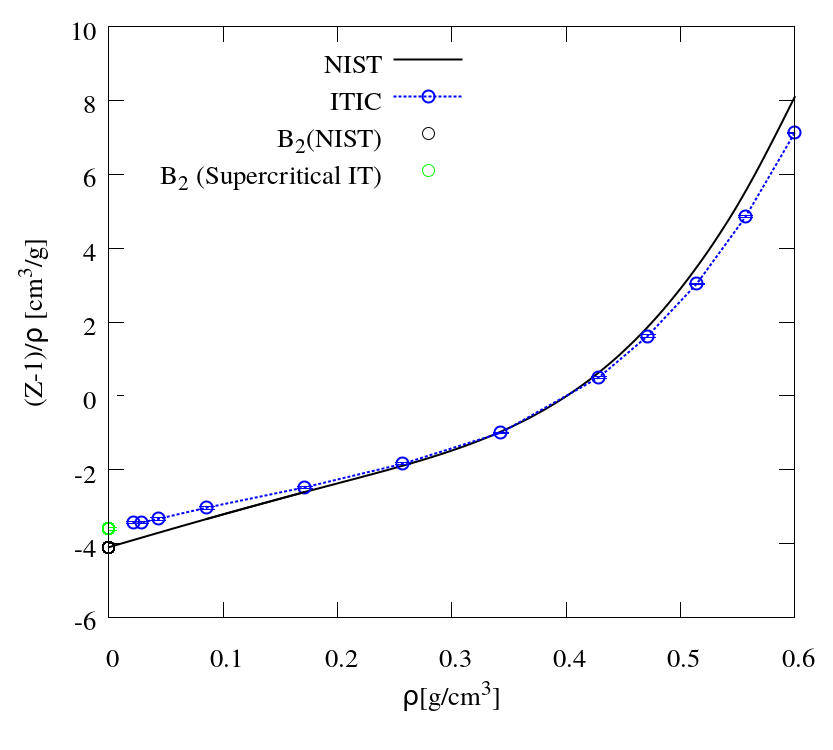
\includegraphics[scale=0.35]{Figures/EXAMPLE-SIM_TraPPE-C2_zrho.png}
\caption{Compressibility factor plot of TraPPE-UA ethane with repect to density. }
\label{fig:EXAMPLE-SIM/TraPPE-C2/zrho}
\end{figure}

\begin{figure}[!htbp]
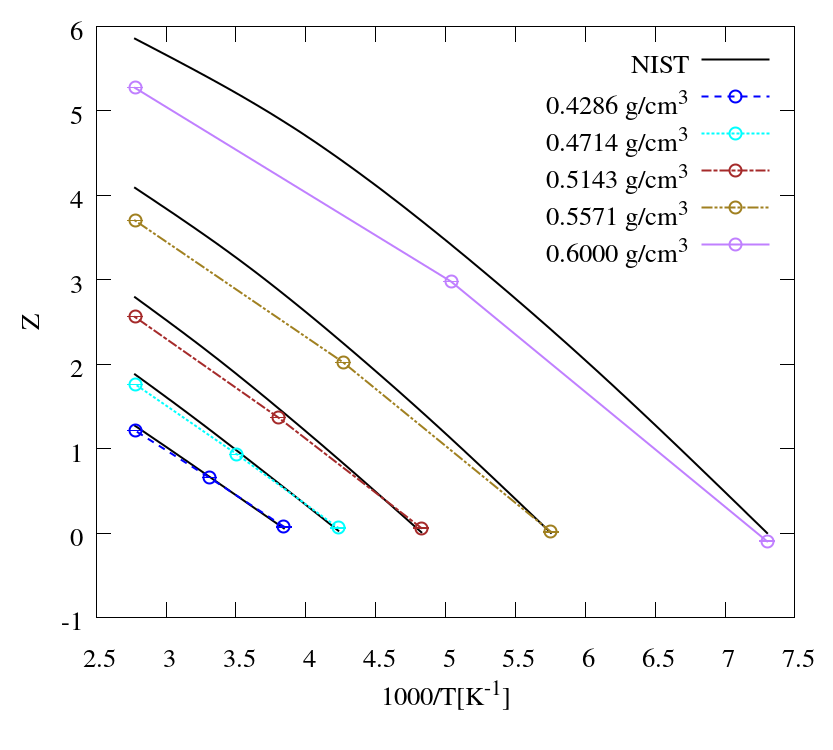
\includegraphics[scale=0.35]{Figures/EXAMPLE-SIM_TraPPE-C2_zt.png}
\caption{Plot of TraPPE-UA ethane isochores at different densities compared to NIST values.}
\label{fig:EXAMPLE-SIM/TraPPE-C2/zt}
\end{figure}

\begin{figure}[!htbp]
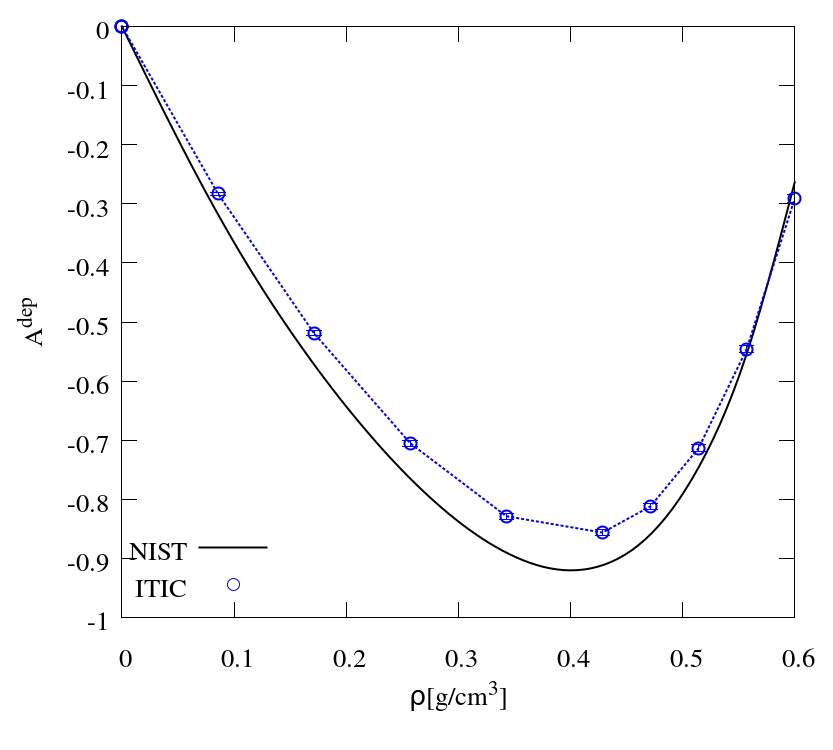
\includegraphics[scale=0.35]{Figures/EXAMPLE-SIM_TraPPE-C2_adep.png}
\caption{Helmholtz energy departure function of TraPPE-UA ethane as a function of density compared to NIST data.}
\label{fig:EXAMPLE-SIM/TraPPE-C2/adep}
\end{figure}

\begin{figure}[!htbp]
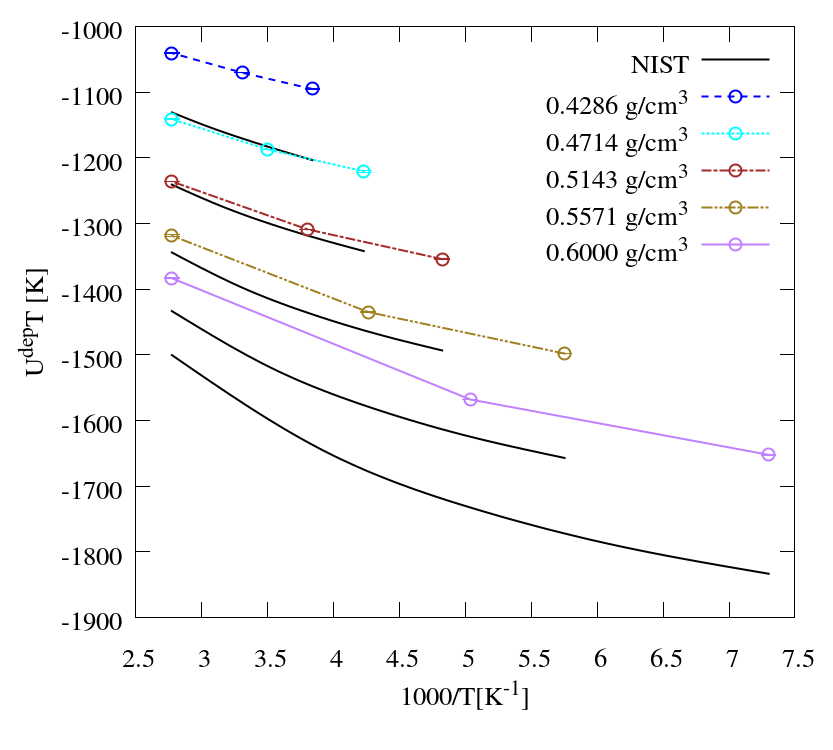
\includegraphics[scale=0.35]{Figures/EXAMPLE-SIM_TraPPE-C2_udep.png}
\caption{Internal energy departure function of TraPPE-UA ethane.}
\label{fig:EXAMPLE-SIM/TraPPE-C2/udep}
\end{figure}

\begin{figure}[!htbp]
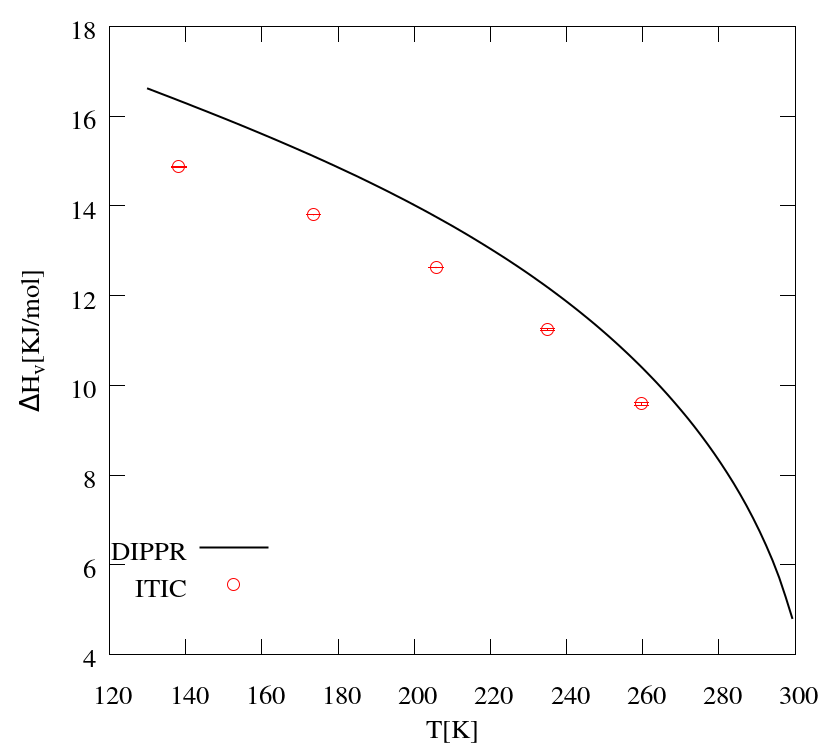
\includegraphics[scale=0.35]{Figures/EXAMPLE-SIM_TraPPE-C2_hvap.png}
\caption{Heat of vaporization of TraPPE-UA ethane.}
\label{fig:EXAMPLE-SIM/TraPPE-C2/hvap}
\end{figure}

\begin{figure}[!htbp]
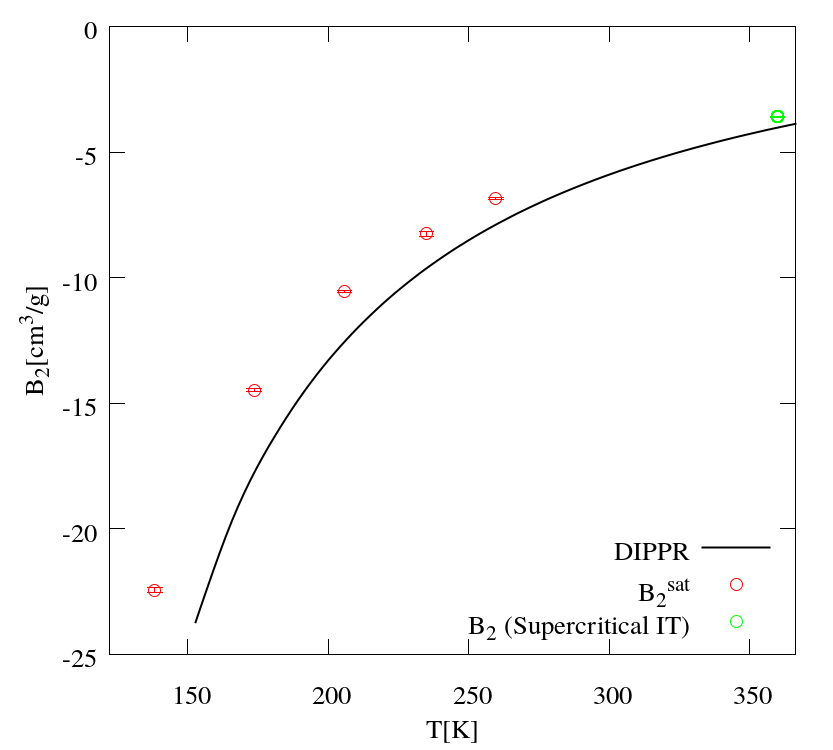
\includegraphics[scale=0.35]{Figures/EXAMPLE-SIM_TraPPE-C2_b2.png}
\caption{Second virial coefficient plot of TraPPE-UA ethane.}
\label{fig:EXAMPLE-SIM/TraPPE-C2/b2}
\end{figure}

%==================================

\begin{figure}[!htbp]
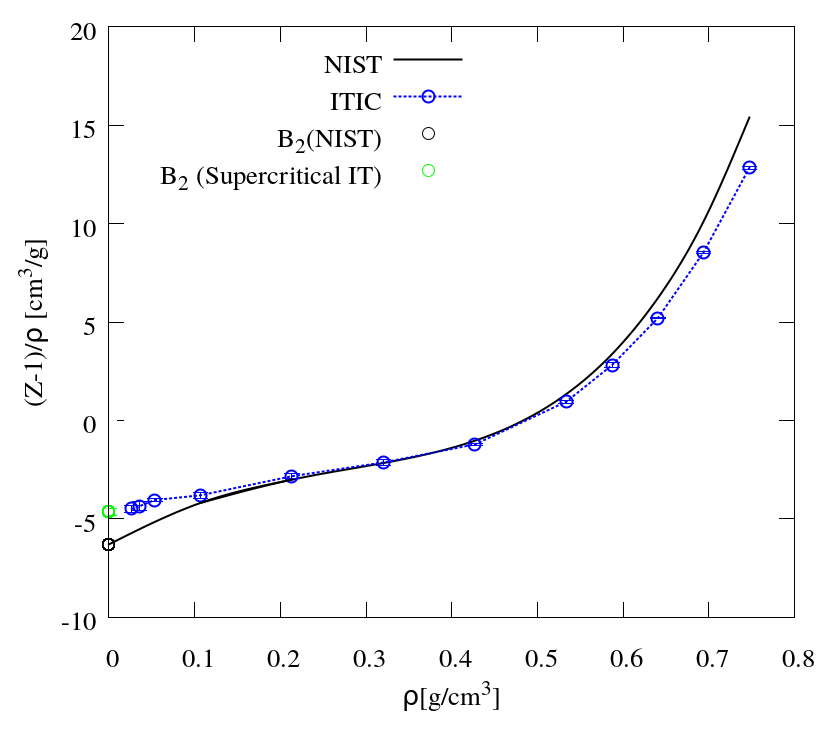
\includegraphics[scale=0.35]{Figures/EXAMPLE-SIM_TraPPE-C12_zrho.png}
\caption{Compressibility factor plot of TraPPE-UA \textit{n}-dodecane with repect to density. }
\label{fig:EXAMPLE-SIM/TraPPE-C12/zrho}
\end{figure}

\begin{figure}[!htbp]
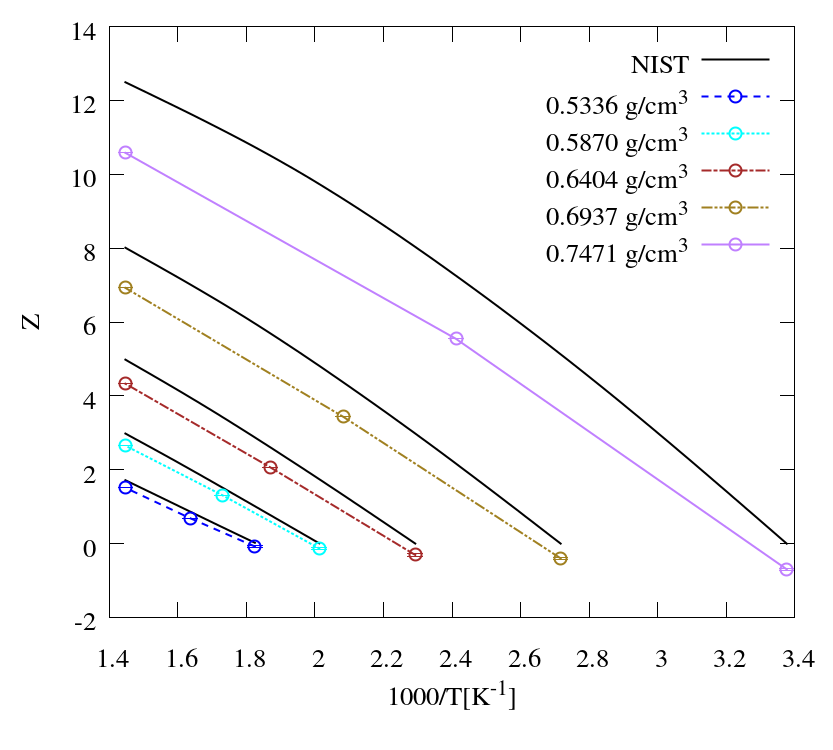
\includegraphics[scale=0.35]{Figures/EXAMPLE-SIM_TraPPE-C12_zt.png}
\caption{Plot of TraPPE-UA \textit{n}-dodecane isochores at different densities compared to NIST values.}
\label{fig:EXAMPLE-SIM/TraPPE-C12/zt}
\end{figure}

\begin{figure}[!htbp]
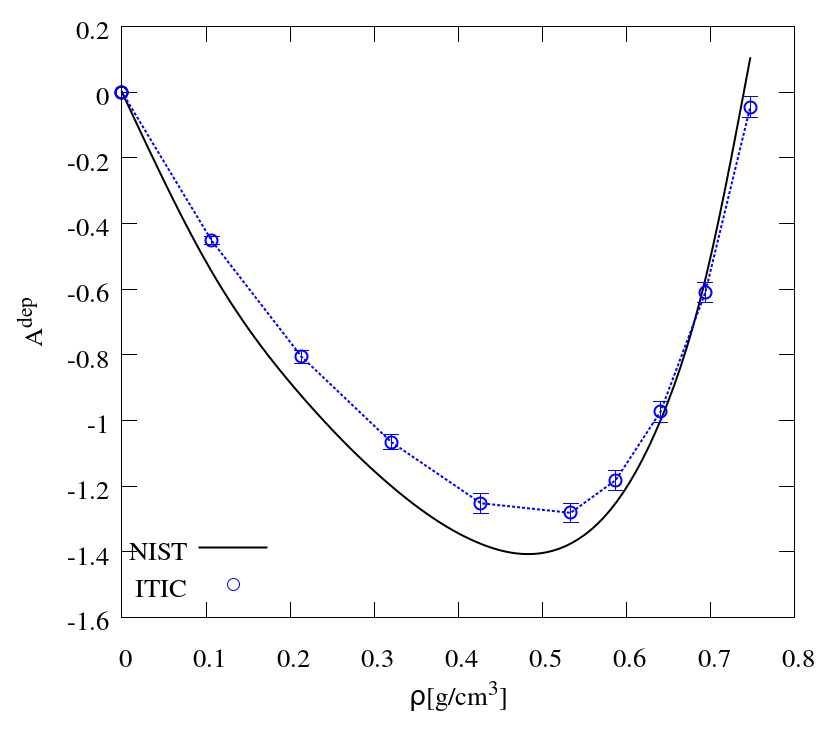
\includegraphics[scale=0.35]{Figures/EXAMPLE-SIM_TraPPE-C12_adep.png}
\caption{Helmholtz energy departure function of TraPPE-UA \textit{n}-dodecane as a function of density compared to NIST data.}
\label{fig:EXAMPLE-SIM/TraPPE-C12/adep}
\end{figure}

\begin{figure}[!htbp]
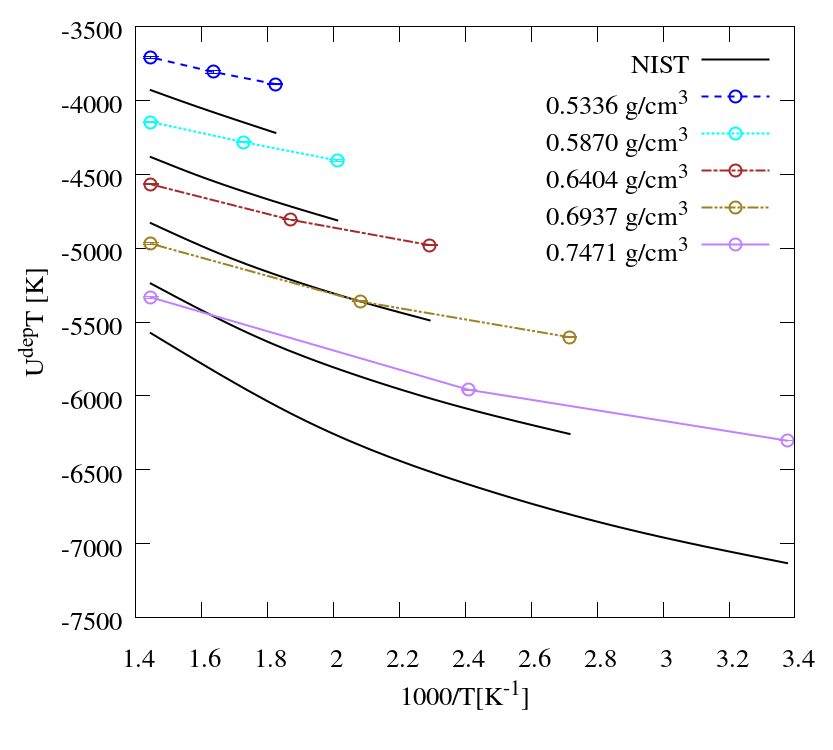
\includegraphics[scale=0.35]{Figures/EXAMPLE-SIM_TraPPE-C12_udep.png}
\caption{Internal energy departure function of TraPPE-UA \textit{n}-dodecane.}
\label{fig:EXAMPLE-SIM/TraPPE-C12/udep}
\end{figure}

\begin{figure}[!htbp]
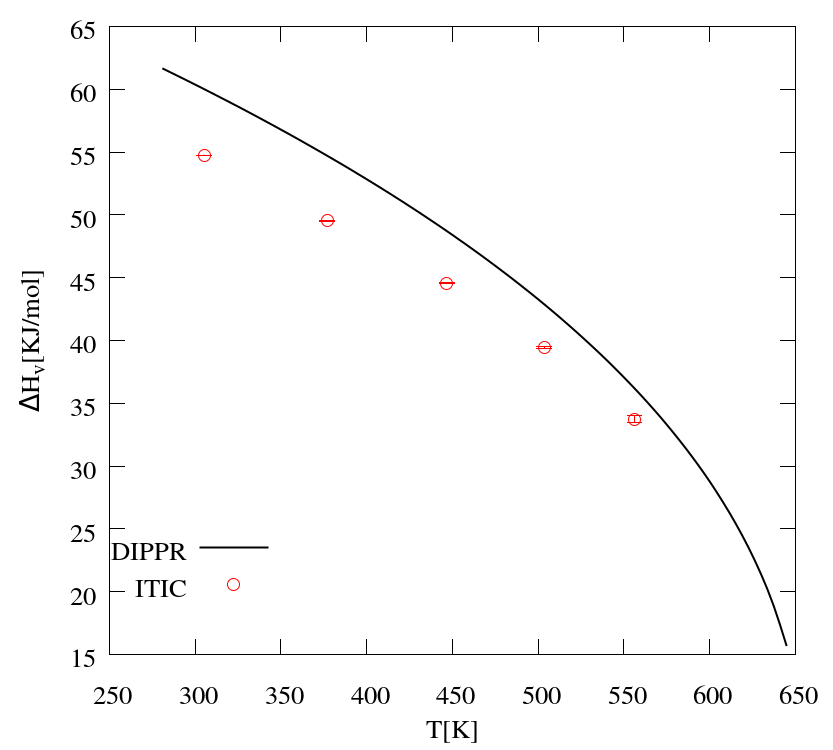
\includegraphics[scale=0.35]{Figures/EXAMPLE-SIM_TraPPE-C12_hvap.png}
\caption{Heat of vaporization of TraPPE-UA \textit{n}-dodecane.}
\label{fig:EXAMPLE-SIM/TraPPE-C12/hvap}
\end{figure}

\begin{figure}[!htbp]
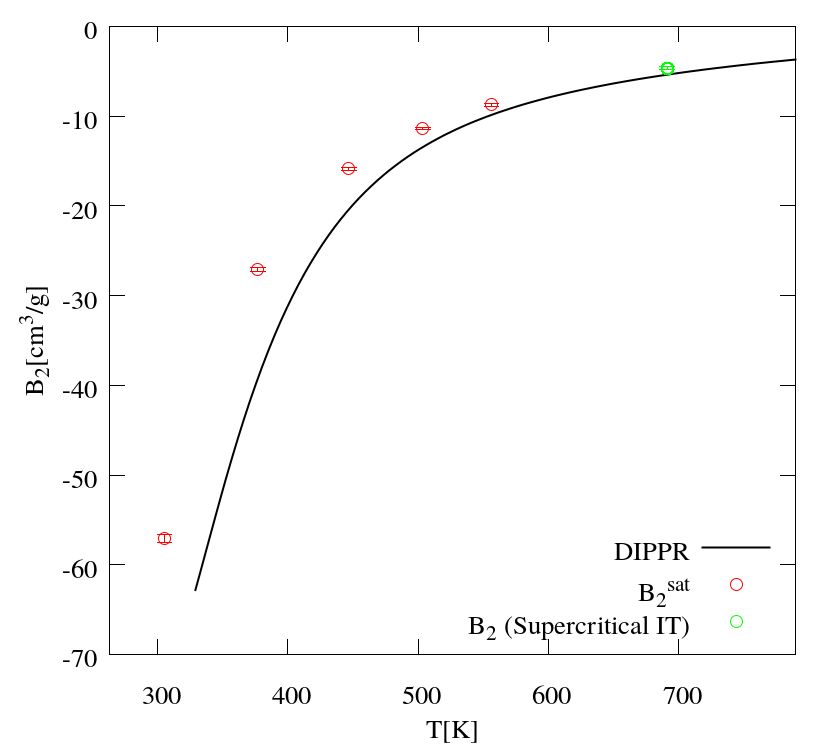
\includegraphics[scale=0.35]{Figures/EXAMPLE-SIM_TraPPE-C12_b2.png}
\caption{Second virial coefficient plot of TraPPE-UA \textit{n}-dodecane.}
\label{fig:EXAMPLE-SIM/TraPPE-C12/b2}
\end{figure}

%=================================================

\begin{figure}[!htbp]
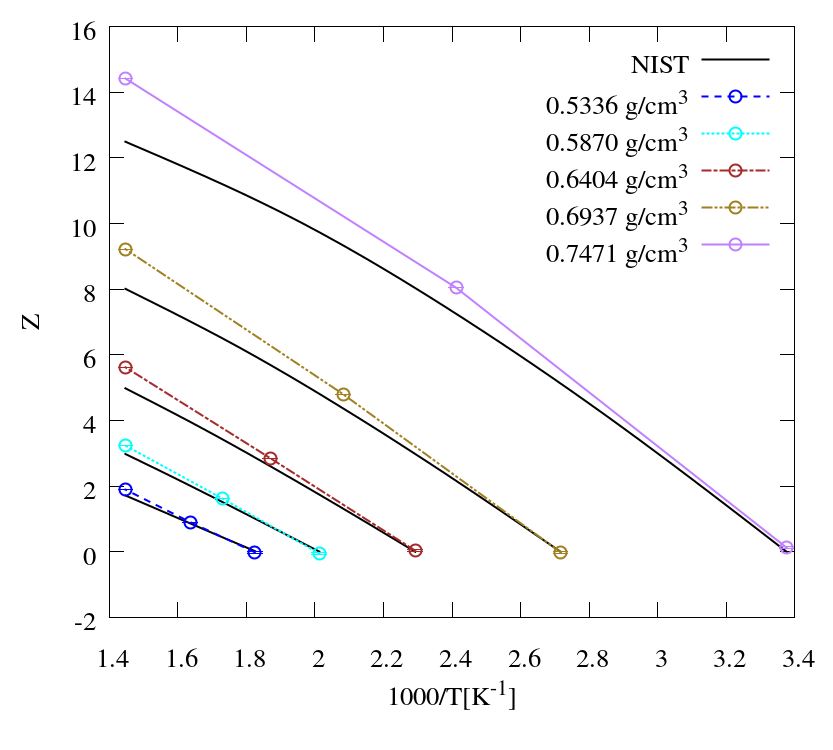
\includegraphics[scale=0.35]{Figures/EXAMPLE-SIM_Mie-C12_zt.png}
\caption{Plot of Mie-UA \textit{n}-dodecane isochores at different densities compared to NIST values.}
\label{fig:EXAMPLE-SIM/Mie-C12/zt}
\end{figure}

\begin{figure}[!htbp]
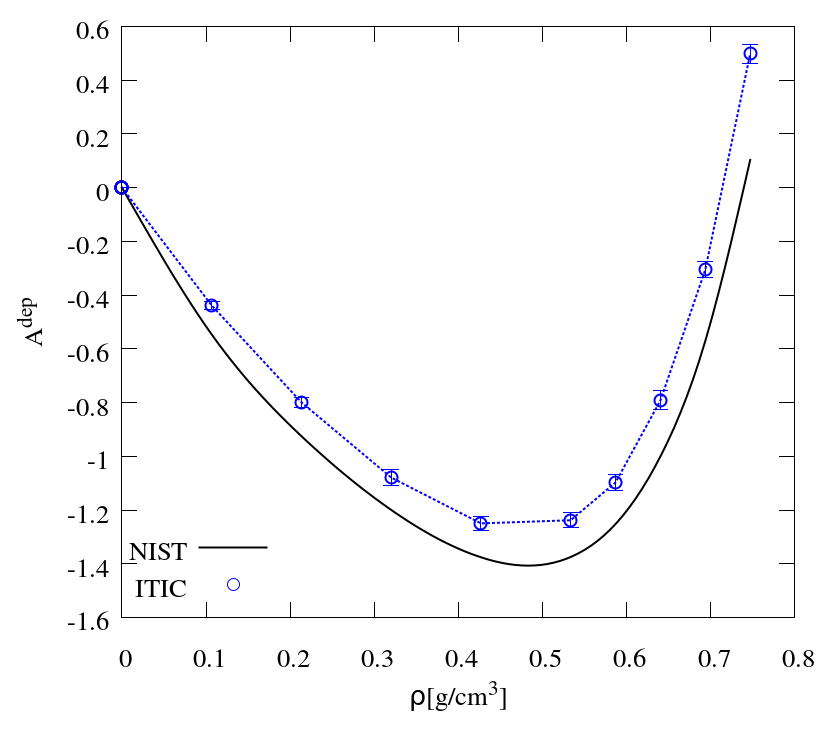
\includegraphics[scale=0.35]{Figures/EXAMPLE-SIM_Mie-C12_adep.png}
\caption{Helmholtz energy departure function of Mie-UA \textit{n}-dodecane as a function of density compared to NIST data.}
\label{fig:EXAMPLE-SIM/Mie-C12/adep}
\end{figure}

\begin{figure}[!htbp]
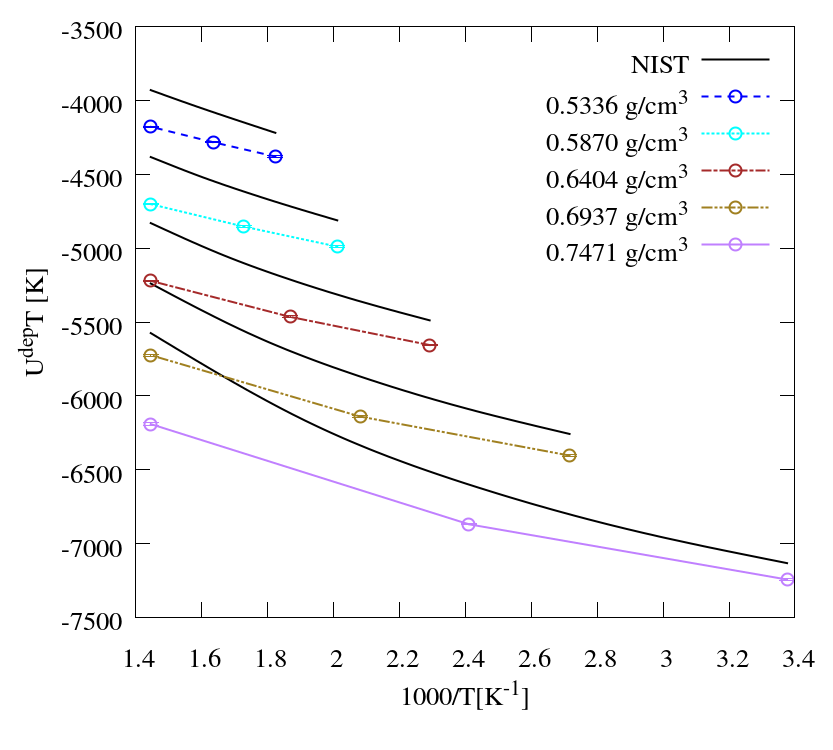
\includegraphics[scale=0.35]{Figures/EXAMPLE-SIM_Mie-C12_udep.png}
\caption{Internal energy departure function of Mie-UA \textit{n}-dodecane.}
\label{fig:EXAMPLE-SIM/Mie-C12/udep}
\end{figure}

\begin{figure}[!htbp]
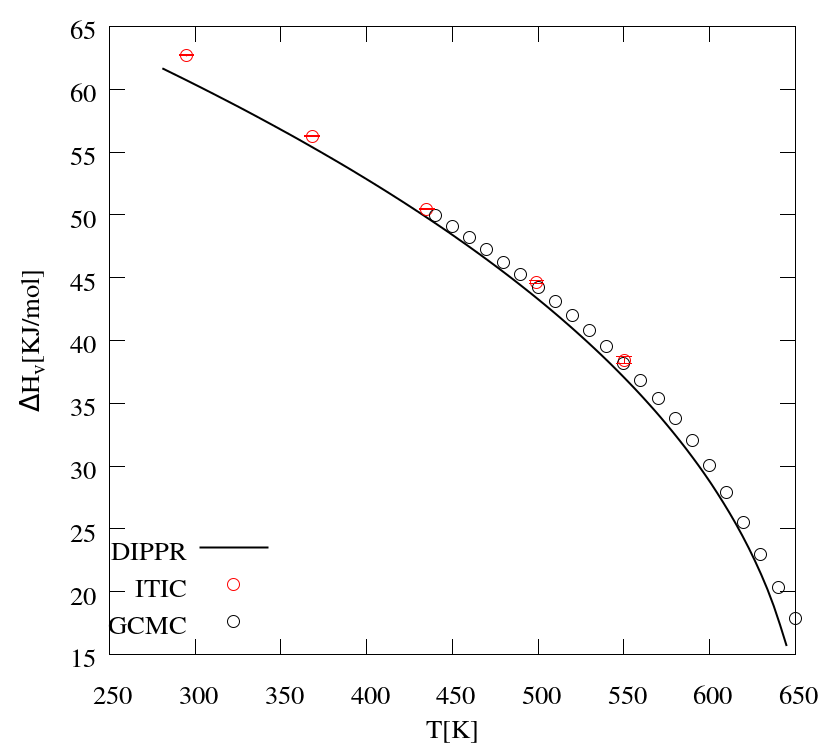
\includegraphics[scale=0.35]{Figures/EXAMPLE-SIM_Mie-C12_hvap.png}
\caption{Heat of vaporization of Mie-UA \textit{n}-dodecane. GCMC data were obtained from Ref.~\onlinecite{Potoff2009}.}
\label{fig:EXAMPLE-SIM/Mie-C12/hvap}
\end{figure}

\begin{figure}[!htbp]
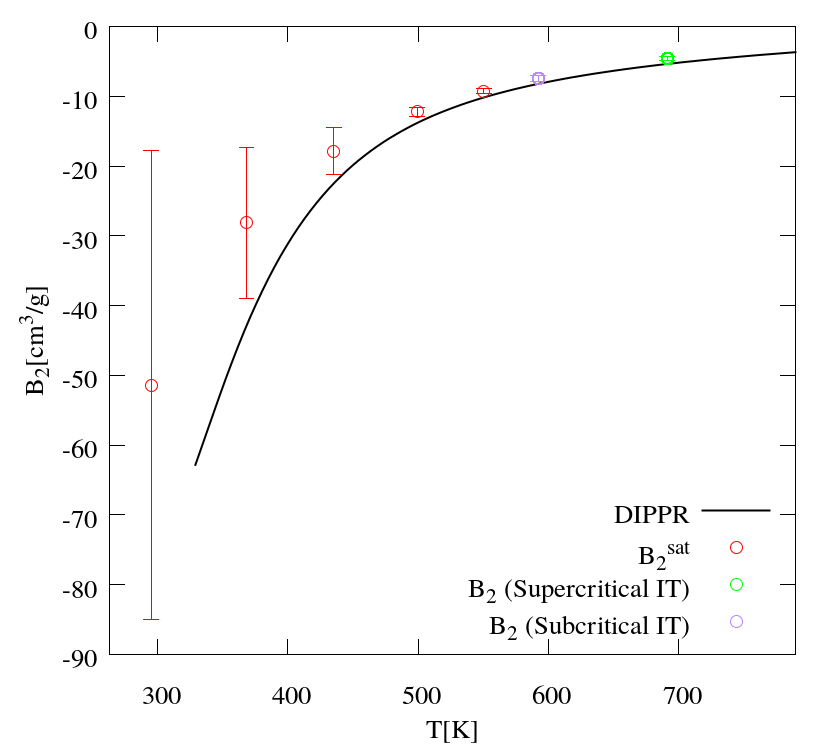
\includegraphics[scale=0.35]{Figures/EXAMPLE-SIM_Mie-C12_b2.png}
\caption{Second virial coefficient plot of Mie-UA \textit{n}-dodecane.}
\label{fig:EXAMPLE-SIM/Mie-C12/b2}
\end{figure}


%==========================================


\begin{figure}[!htbp]
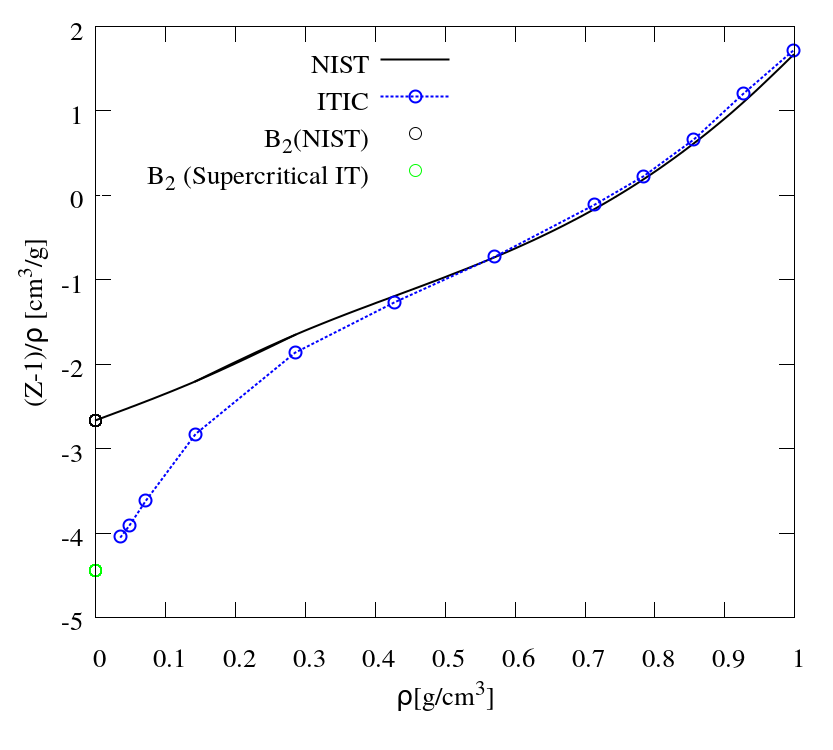
\includegraphics[scale=0.35]{Figures/EXAMPLE-SIM_TIP4P05_zrho.png}
\caption{Compressibility factor plot of TIP4P/2005 water with repect to density. }
\label{fig:EXAMPLE-SIM/TIP4P05/zrho}
\end{figure}

\begin{figure}[!htbp]
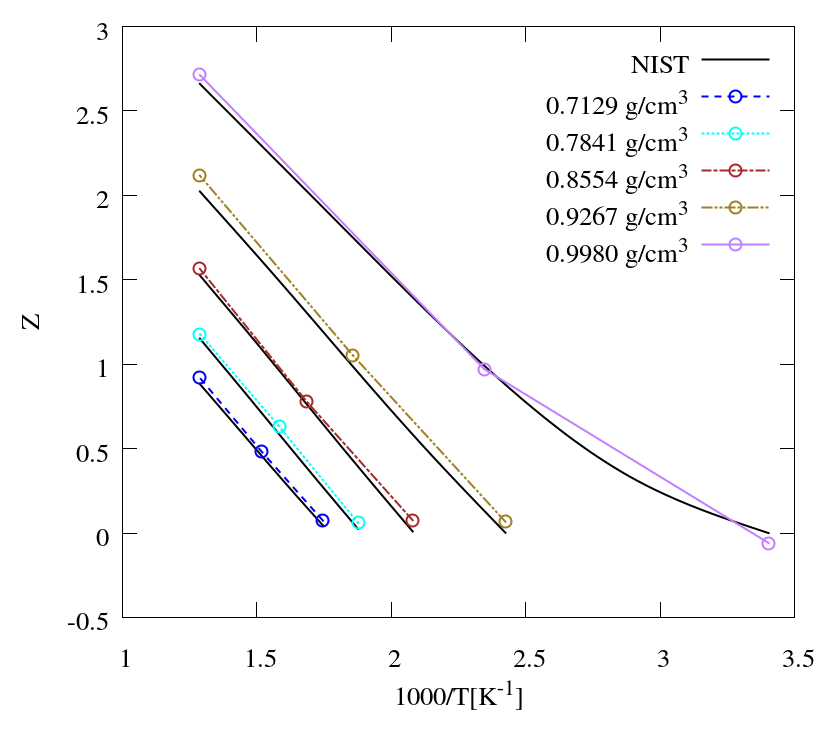
\includegraphics[scale=0.35]{Figures/EXAMPLE-SIM_TIP4P05_zt.png}
\caption{Plot of TIP4P/2005 isochores at different densities compared to NIST values.}
\label{fig:EXAMPLE-SIM/TIP4P05/zt}
\end{figure}

\begin{figure}[!htbp]
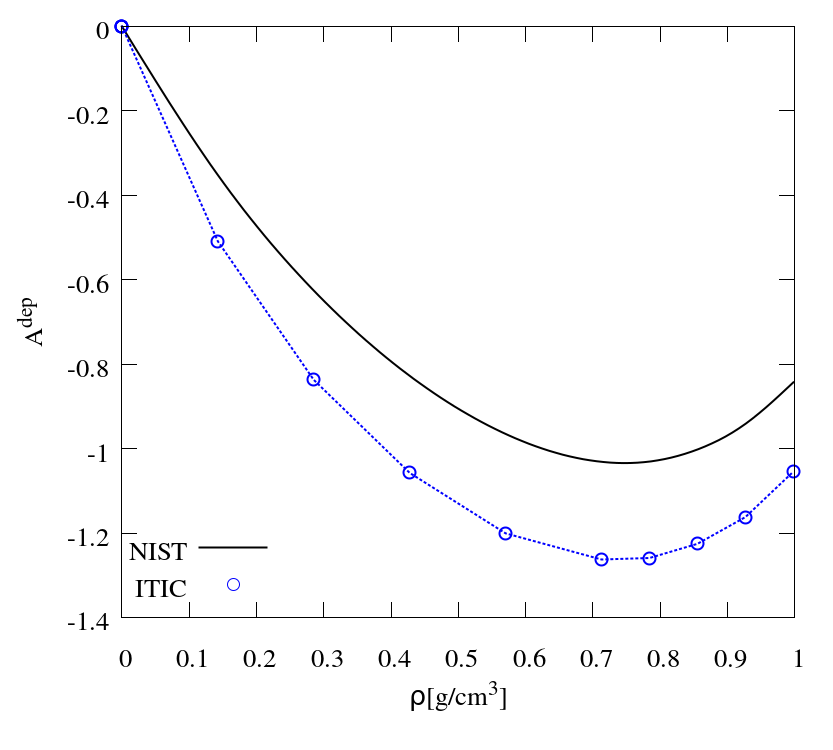
\includegraphics[scale=0.35]{Figures/EXAMPLE-SIM_TIP4P05_adep.png}
\caption{Helmholtz energy departure function of TIP4P/2005 water as a function of density compared to NIST data.}
\label{fig:EXAMPLE-SIM/TIP4P05/adep}
\end{figure}

\begin{figure}[!htbp]
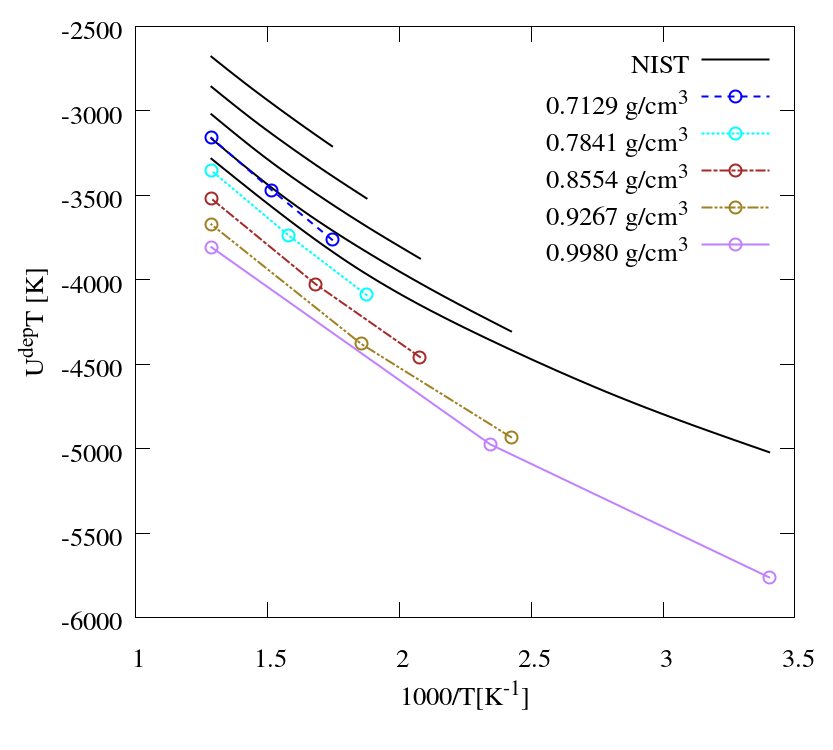
\includegraphics[scale=0.35]{Figures/EXAMPLE-SIM_TIP4P05_udep.png}
\caption{Internal energy departure function of TIP4P/2005 water.}
\label{fig:EXAMPLE-SIM/TIP4P05/udep}
\end{figure}

\begin{figure}[!htbp]
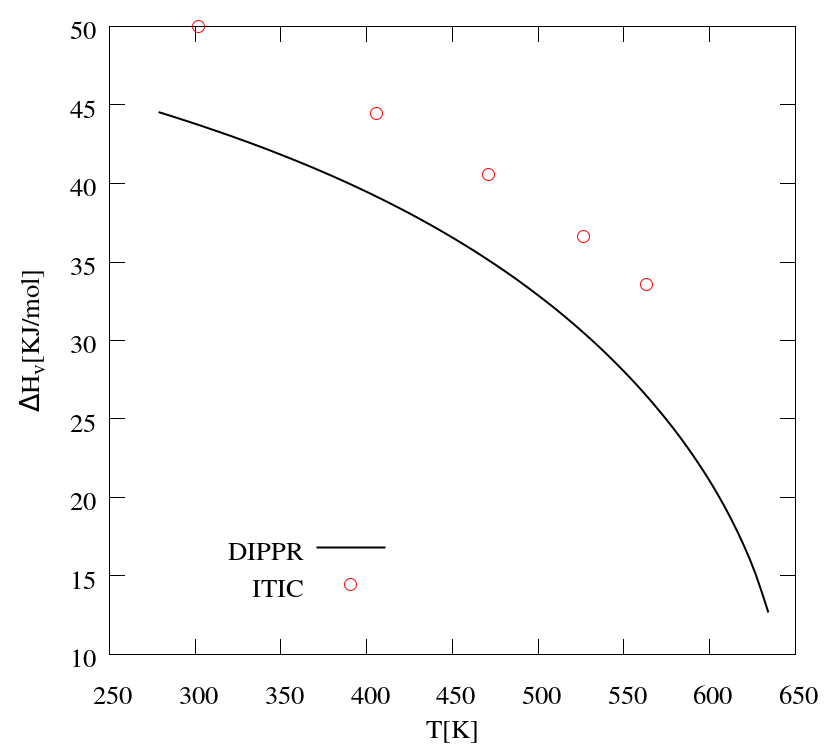
\includegraphics[scale=0.35]{Figures/EXAMPLE-SIM_TIP4P05_hvap.png}
\caption{Heat of vaporization of TIP4P/2005 water.}
\label{fig:EXAMPLE-SIM/TIP4P05/hvap}
\end{figure}

\begin{figure}[!htbp]
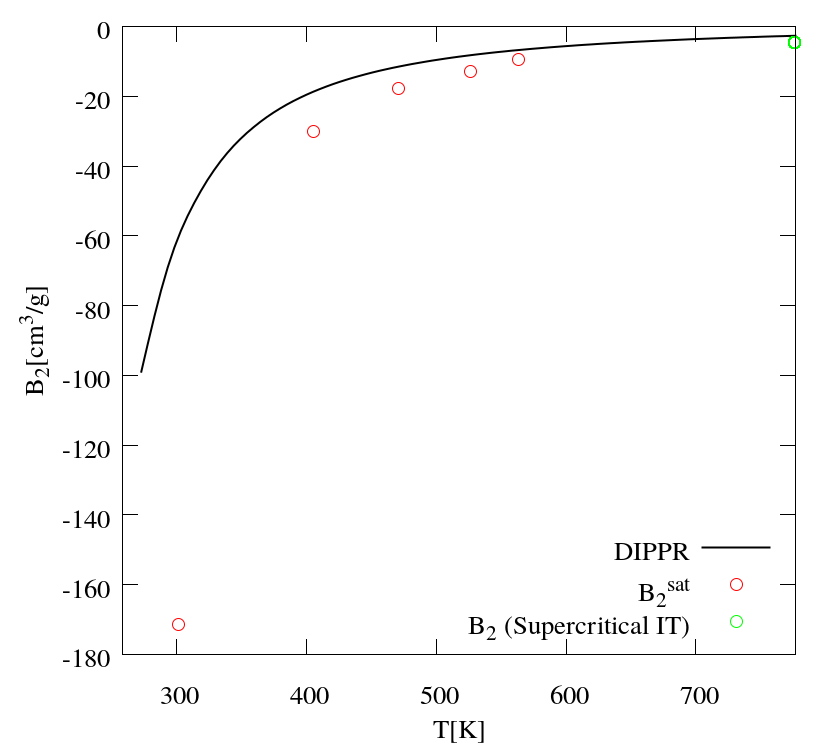
\includegraphics[scale=0.35]{Figures/EXAMPLE-SIM_TIP4P05_b2.png}
\caption{Second virial coefficient plot of TIP4P/2005 water.}
\label{fig:EXAMPLE-SIM/TIP4P05/b2}
\end{figure}

\newpage
\clearpage
\bibliography{ITIC-Paper}
\end{document}
